\begin{figure}[htbp]
    \centering
    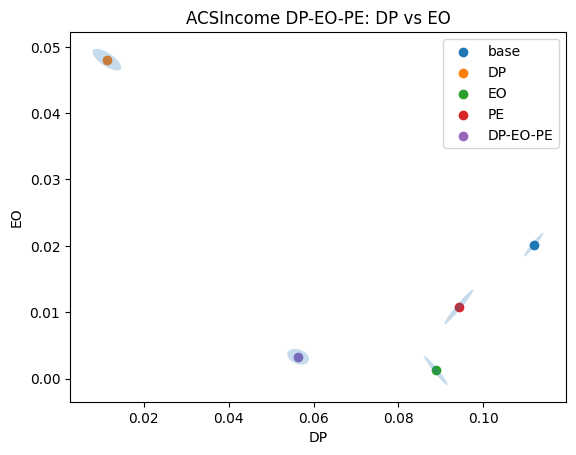
\includegraphics[width=0.45\textwidth]{assets/combined/ACSIncome_DP-EO-PE_DP-EO.png}
    \hfill
    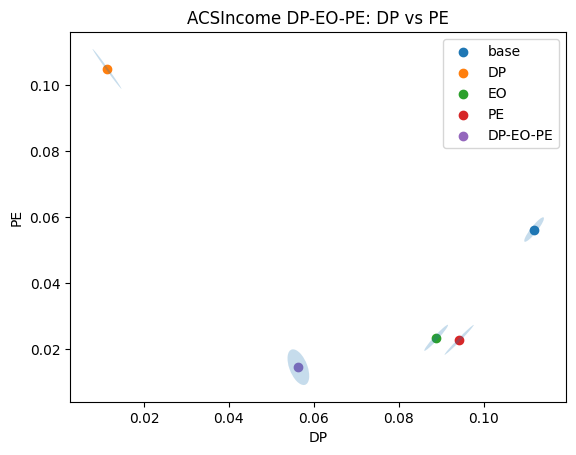
\includegraphics[width=0.45\textwidth]{assets/combined/ACSIncome_DP-EO-PE_DP-PE.png}
    \hfill
    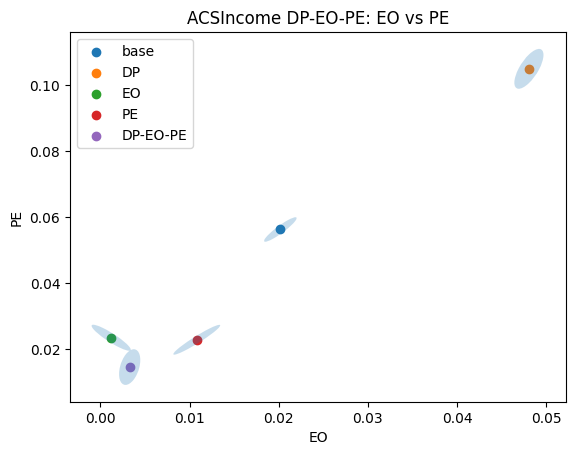
\includegraphics[width=0.45\textwidth]{assets/combined/ACSIncome_DP-EO-PE_EO-PE.png}
    \caption{Violation measures of DP, EO and PE for an unconstrained baseline model, single constrained models and a combined constrained model. Averages were calculated from 5 samples runs.}
    \label{fig:triple1}
\end{figure}
        
\begin{figure}[htbp]
    \centering
    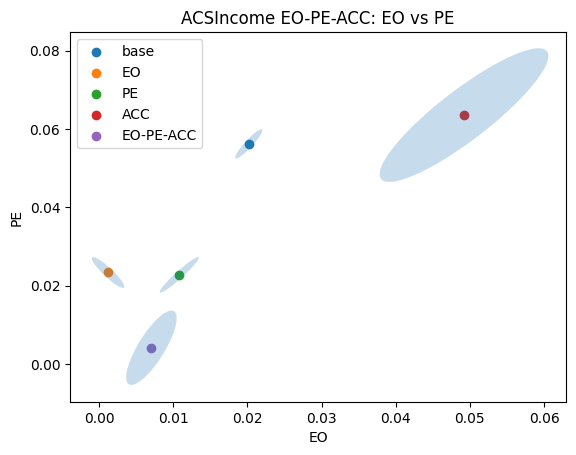
\includegraphics[width=0.45\textwidth]{assets/combined/ACSIncome_EO-PE-ACC_EO-PE.png}
    \hfill
    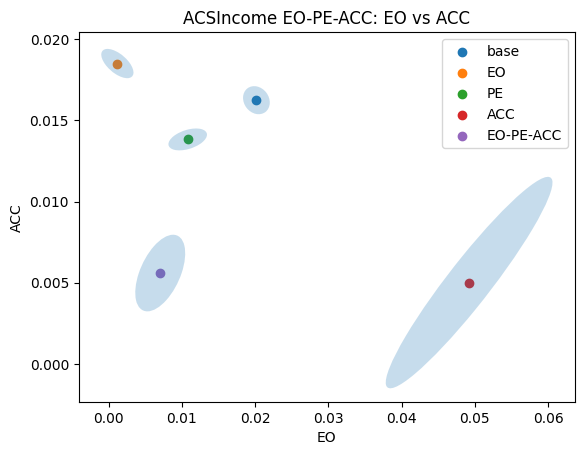
\includegraphics[width=0.45\textwidth]{assets/combined/ACSIncome_EO-PE-ACC_EO-ACC.png}
    \hfill
    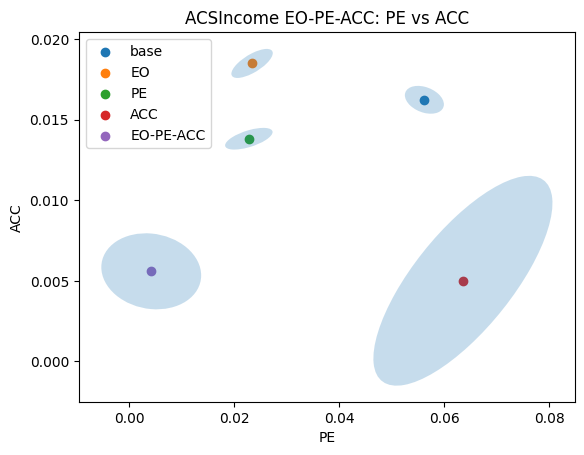
\includegraphics[width=0.45\textwidth]{assets/combined/ACSIncome_EO-PE-ACC_PE-ACC.png}
    \caption{Violation measures of EO, PE and ACC for an unconstrained baseline model, single constrained models and a combined constrained model. Averages were calculated from 5 samples runs.}
\end{figure}
        
\begin{figure}[htbp]
    \centering
    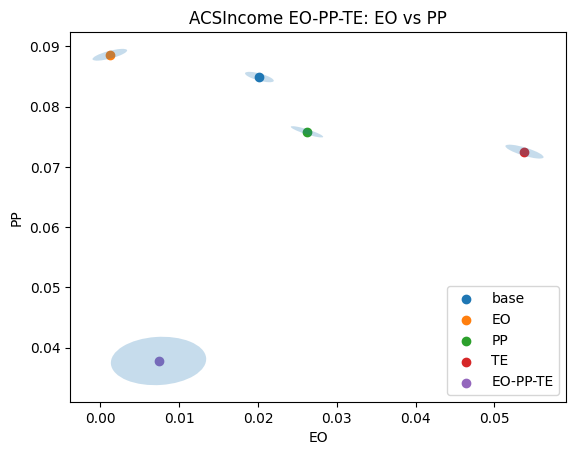
\includegraphics[width=0.45\textwidth]{assets/combined/ACSIncome_EO-PP-TE_EO-PP.png}
    \hfill
    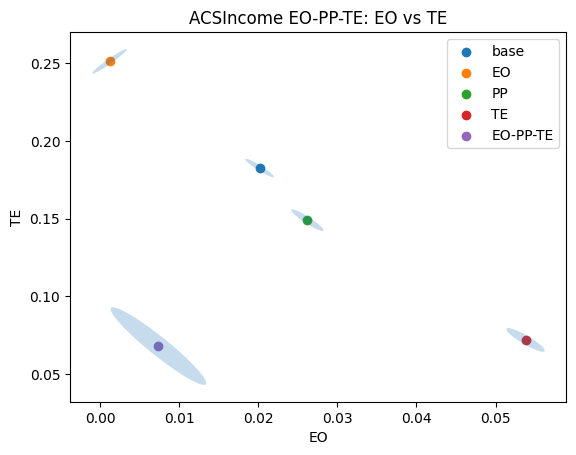
\includegraphics[width=0.45\textwidth]{assets/combined/ACSIncome_EO-PP-TE_EO-TE.png}
    \hfill
    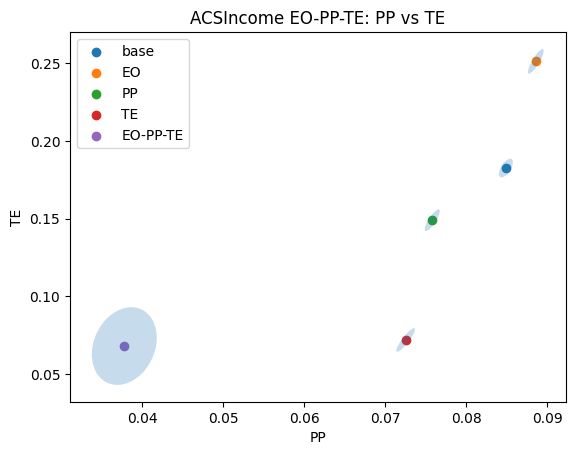
\includegraphics[width=0.45\textwidth]{assets/combined/ACSIncome_EO-PP-TE_PP-TE.png}
    \caption{Violation measures of EO, PP and TE for an unconstrained baseline model, single constrained models and a combined constrained model. Averages were calculated from 5 samples runs.}
    \label{fig:EO-PP-TE}
\end{figure}
        
\begin{figure}[htbp]
    \centering
    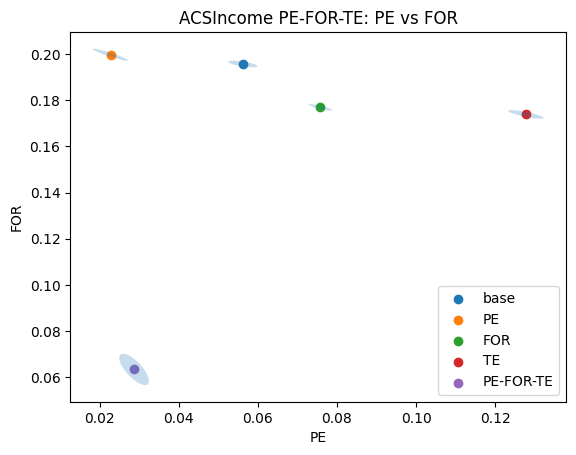
\includegraphics[width=0.45\textwidth]{assets/combined/ACSIncome_PE-FOR-TE_PE-FOR.png}
    \hfill
    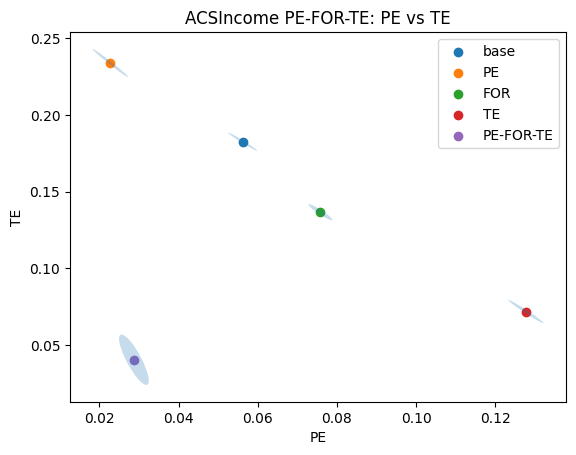
\includegraphics[width=0.45\textwidth]{assets/combined/ACSIncome_PE-FOR-TE_PE-TE.png}
    \hfill
    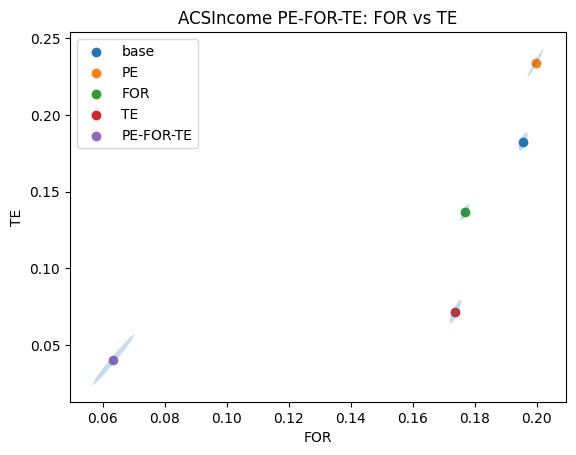
\includegraphics[width=0.45\textwidth]{assets/combined/ACSIncome_PE-FOR-TE_FOR-TE.png}
    \caption{Violation measures of PE, FOR and TE for an unconstrained baseline model, single constrained models and a combined constrained model. Averages were calculated from 5 samples runs.}
\end{figure}
        
\begin{figure}[htbp]
    \centering
    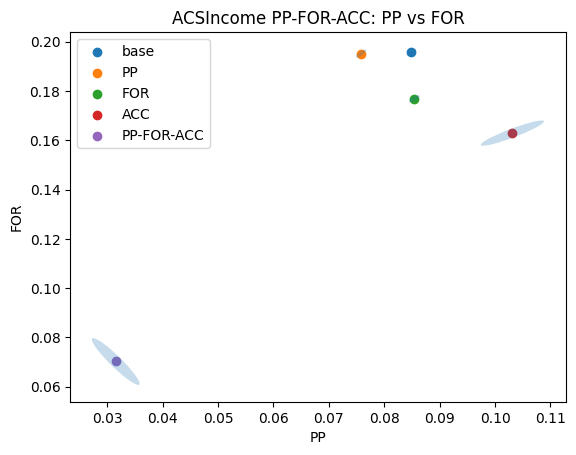
\includegraphics[width=0.45\textwidth]{assets/combined/ACSIncome_PP-FOR-ACC_PP-FOR.png}
    \hfill
    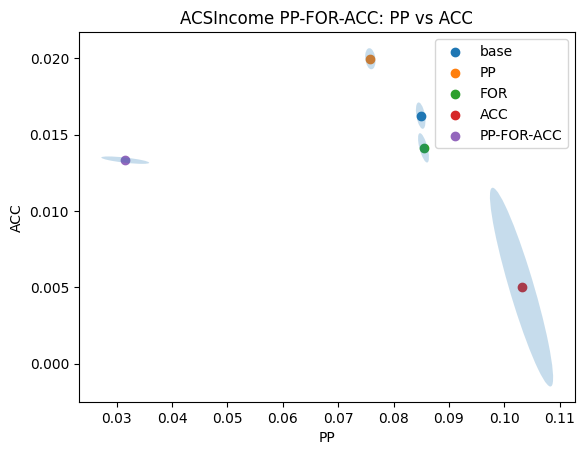
\includegraphics[width=0.45\textwidth]{assets/combined/ACSIncome_PP-FOR-ACC_PP-ACC.png}
    \hfill
    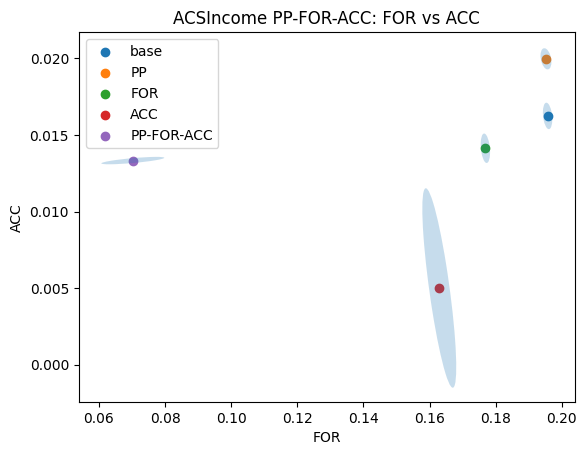
\includegraphics[width=0.45\textwidth]{assets/combined/ACSIncome_PP-FOR-ACC_FOR-ACC.png}
    \caption{Violation measures of PP, FOR and ACC for an unconstrained baseline model, single constrained models and a combined constrained model. Averages were calculated from 5 samples runs.}
    \label{fig:triple5}
    \label{fig:PP-FOR-ACC}
\end{figure}